\documentclass[10pt,conference]{IEEEtran}
\IEEEoverridecommandlockouts
% The preceding line is only needed to identify funding in the first footnote. If that is unneeded, please comment it out.

\usepackage{cite}
\usepackage{amsmath,amssymb,amsfonts}
\usepackage{algorithmic}
\usepackage{graphicx}
\usepackage{textcomp}
\usepackage{xcolor}
\usepackage{balance}
\def\BibTeX{{\rm B\kern-.05em{\sc i\kern-.025em b}\kern-.08em
    T\kern-.1667em\lower.7ex\hbox{E}\kern-.125emX}}

\newcommand{\mytitle}{Input Debugging via Rich %and Fast
Failure Feedback}
\renewcommand{\mytitle}{Repairing Inputs}
\renewcommand{\mytitle}{Repairing Inputs with Input Synthesis}
\renewcommand{\mytitle}{Repairing Inputs via Synthesis}
%\renewcommand{\mytitle}{Input Repair via Synthesis and Lightweight \\ Error Feedback}
\edef\mytitle{\mytitle\\Supplementary Material}


\usepackage{listings}
\lstset{ % General setup for the package
    language=Python,
    %basicstyle=\small\sffamily,
    %basicstyle=\footnotesize,  % *Please* use a monospaced font -- AZ
    basicstyle=\footnotesize\ttfamily,
    numbers=left,
    numberstyle=\tiny,
    frame=none,
    tabsize=4,
    columns=flexible,
    keepspaces=true,
    showstringspaces=false,
    showtabs=false,
    keepspaces,
    commentstyle=\color{green},
    keywordstyle=\color{blue}
}
\usepackage{xspace}
\usepackage{array,multirow,graphicx}
\usepackage{float}
\usepackage{framed}
\usepackage{tikz,pgfplots,pgfplotstable}
\usetikzlibrary{calc,positioning,patterns}
\usepackage{hyperref}
\usepackage{cleveref}
\usepackage{boxedminipage}
\usepackage[inline]{enumitem}
\setlength{\FrameSep}{3pt}
\setlength{\OuterFrameSep}{2pt}
\newenvironment{result}{\begin{framed}\centering\it}{\end{framed}}

%% Identifiers
\def\|#1|{\textit{#1}}
\def\<#1>{\texttt{#1}}

\newcounter{todocounter}
\newcommand{\todo}[1]{\marginpar{$|$}\textcolor{red}{\stepcounter{todocounter}\footnote[\thetodocounter]{\textcolor{red}{\textbf{TODO }}\textit{#1}}}}
%\newcommand{\repl}[2]{\textcolor{red}{\textbf{REPLACE }\st{#1} \textit{#2}}}
%\newcommand{\rem}[1]{\textcolor{red}{\textbf{REMOVED }\st{#1}}}
\newcommand{\done}[1]{\marginpar{$*$}\textcolor{green}{\stepcounter{todocounter}\footnote[\thetodocounter]{\textcolor{black}{\textbf{DONE }}\textit{#1}}}}

% \newcommand{\todo}[1]{\textcolor{red}{\textbf{TODO: }\emph{#1}}}
% \newcommand{\com}[1]{\textcolor{orange}{\textbf{COMMENT: }\emph{#1}}}
\newcommand{\recheck}[1]{\textcolor{red}{#1}}
%\newcommand{\revise}[1]{\textcolor{blue}{#1}}
\newcommand{\revise}[1]{#1}

\renewcommand{\done}[1]{} % comment to see responses.

\IfFileExists{SUBMIT}{
\renewcommand{\todo}[1]{}
\renewcommand{\done}[1]{}
%\renewcommand{\rem}[1]{}
%\renewcommand{\theendnotes}{}
}{
}

%--

% Own commands
\newcommand{\dd}{\textit{dd}\xspace}
\newcommand{\ddmin}{\textit{ddmin}\xspace}
%\newcommand{\ddmax}{\textit{ddmax}\xspace}
\newcommand{\test}{\textit{test}\xspace}
%\newcommand{\ddmaxg}{\textit{syntactic ddmax}\xspace}

\usepackage{pifont}
\newcommand{\pass}{\text{\ding{52}}\xspace}
\newcommand{\fail}{\text{\ding{56}}\xspace}
% \newcommand{\unresolved}{\textbf{?}}
\newcommand{\unresolved}{\lower0.1ex\hbox{\includegraphics*[height=1.7ex]{question.pdf}}}


\newcommand{\cpass}{{c_{\scriptscriptstyle \pass}}}
\newcommand{\cfail}{{c_{\scriptscriptstyle \fail}}}
\newcommand{\dpass}{{c'_{\scriptscriptstyle \pass}}}
\newcommand{\dfail}{{c'_{\scriptscriptstyle \fail}}}

%--

\newcommand{\approach}{\textsc{FSynth}\xspace}
\def\bfr{bFuzzerRepairer\xspace}
\def\ddmin{DDMin\xspace}
\newcommand{\ddmax}{\textit{DDMax}\xspace}
\newcommand{\ddmaxg}{\textit{DDmaxG}\xspace}
\newcommand{\bsimple}{\textit{bsimple}\xspace}
\newcommand{\brepair}{\textsc{FSynth}\xspace}

\tikzset{inlinenode/.style={draw=white,text=black,fill=light-gray,inner sep=.1em,outer sep=0em}}
\newcommand{\inlinenode}[1]{\text{\hspace{.1em}\tikz[baseline=(n.base)]{\node[inlinenode] (n) {\strut \hspace*{.3em}#1\hspace*{.3em}};}\hspace{.1em}}}
\newcommand{\inlinetext}[1]{\text{\hspace{.1em}\tikz[baseline=(n.base)]{\node[inlinenode] (n) {\strut \hspace*{.3em}\letterboxed{#1}\hspace*{.3em}};}\hspace{.1em}}}
\newcommand*\circled[1]{\tikz[baseline=(char.base)]{
            \node[shape=circle,draw,inner sep=0.3pt] (char) {#1};}}

\tikzset{%
simpletext/.style={draw=none,text=black,font=\normalfont\normalsize,align=center},
gparsetreenode/.style={minimum width=6mm,minimum height=5mm},
lparsetreenode/.style={gparsetreenode,simpletext,rectangle,draw=white,fill=white,align=center},
lparsetreeerrornode/.style={lparsetreenode,font=\bfseries},
lparsetreephantomnode/.style={gparsetreenode,edge from parent/.append style={draw=none},shape=coordinate,minimum width=15mm},
lparsetreestrikethrough/.style={draw=black,thick},
lparsetreedeletednode/.style={lparsetreenode,append after command={\pgfextra \draw[lparsetreestrikethrough] (\tikzlastnode.north west) -- (\tikzlastnode.south east); \draw[lparsetreestrikethrough] (\tikzlastnode.north east) -- (\tikzlastnode.south west);\endpgfextra}},
lparsetree/.style={node distance=5mm,level distance=10mm,every node/.style={lparsetreenode},edge from parent/.style={draw=black,-latex,shorten >=.5mm}
},
lflowchartnode/.style={lparsetreenode,draw=black,rounded corners=.5pt},
blockdiagramlines/.style={draw,stroke=black,line width=1.2pt},
blockdiagramarrow/.style={blockdiagramlines,->},
blockdiagramdashedarrow/.style={blockdiagramarrow,dashed},
blockdiagramannot/.style={blockdiagramlines,text=black,align=center},
blockdiagramblock/.style={lflowchartnode,blockdiagramannot,minimum width=1.5cm,minimum height=0.5cm,text width=1.9cm},
blockdiagrammicroblock/.style={blockdiagramannot,font=\tiny,minimum width=1.5cm,minimum height=.5cm,rounded corners=.5pt},
blockdiagramarrowcaption/.style={font=\scriptsize\sffamily,inner sep=1.5pt,text=black},
blockdiagramouterbox/.style={blockdiagramlines,densely dotted,line width=.7pt},
blockdiagramouterboxcaption/.style={blockdiagramarrowcaption,font=\itshape\scriptsize,inner sep=1pt},
pics/numbering/.style args={#1}{code={
    \node[draw=black,shape=circle,fill=white,text=black,font=\ttfamily\scriptsize,inner sep=1pt,text width=8pt,align=center,outer sep=0] (-number) {#1};
}}}

% Boxes around letters
\definecolor{light-gray}{gray}{0.87}
\makeatletter
\newcommand\letterboxed[1]{%
\setlength{\fboxsep}{0pt}%
  \@tfor\@ii:=#1\do{%
    \fcolorbox{white}{light-gray}{\texttt{\strut\@ii}}%
  }%
}

\newcommand\letterboxedinTable[1]{%
\setlength{\fboxsep}{0pt}%
  \@tfor\@ii:=#1\do{%
    \fcolorbox{white}{light-gray}{\tiny \texttt{\strut\@ii}}%
  }%
}

\makeatother



\usepackage[utf8]{inputenc}

\begin{document}

\title{\mytitle}
%\author{\IEEEauthorblockN{1\textsuperscript{st} Given Name Surname}
%\IEEEauthorblockA{\textit{dept. name of organization (of Aff.)} \\
%\textit{name of organization (of Aff.)}\\
%City, Country \\
%email address or ORCID}
%\and
%\IEEEauthorblockN{2\textsuperscript{nd} Given Name Surname}
%\IEEEauthorblockA{\textit{dept. name of organization (of Aff.)} \\
%\textit{name of organization (of Aff.)}\\
%City, Country \\
%email address or ORCID}
%\and
%\IEEEauthorblockN{3\textsuperscript{rd} Given Name Surname}
%\IEEEauthorblockA{\textit{dept. name of organization (of Aff.)} \\
%\textit{name of organization (of Aff.)}\\
%City, Country \\
%email address or ORCID}
%\and
%\IEEEauthorblockN{4\textsuperscript{th} Given Name Surname}
%\IEEEauthorblockA{\textit{dept. name of organization (of Aff.)} \\
%\textit{name of organization (of Aff.)}\\
%City, Country \\
%email address or ORCID}
%\and
%\IEEEauthorblockN{5\textsuperscript{th} Given Name Surname}
%\IEEEauthorblockA{\textit{dept. name of organization (of Aff.)} \\
%\textit{name of organization (of Aff.)}\\
%City, Country \\
%email address or ORCID}
%\and
%\IEEEauthorblockN{6\textsuperscript{th} Given Name Surname}
%\IEEEauthorblockA{\textit{dept. name of organization (of Aff.)} \\
%\textit{name of organization (of Aff.)}\\
%City, Country \\
%email address or ORCID}
%}
\maketitle

\begin{figure}
%\begin{lstlisting}[caption=binary search,label={lst:bsearch}]
\begin{lstlisting}
def binary_search(inputstr, left=0, 
                right=len(inputstr)-1):
  if not inputstr: return left
  if is_incomplete(Repair(inputstr, right)):
    return len(inputstr)-1
  while left + 1 < right:
    middle = (left + right) // 2
    if is_incomplete(Repair(inputstr, middle)):
      left = middle
    else:
      right = middle
  return left
\end{lstlisting}
\caption{Code showing the binary search that is performed at the beginning of the repair}
\end{figure}

\begin{figure}
%\begin{lstlisting}[caption=Sampling,label={lst:sampling}]
\begin{lstlisting}
def sample_items_by_mask(items):
  masks = {}
  for i in items:
    key = (i.mask, i.boundary, i.inputstr[i.boundary-1])
    if i.mask not in masks: masks[key] = []
    masks[key].append(i)

  sampled = []
  for key in masks:
    if len(masks[key]) < MAX_NUM_PER_MASK:
      res = masks[key]
    else:
      res = random.sample(masks[key], MAX_NUM_PER_MASK)
    sampled.extend(res)
  return filter_best(sampled)

def filter_best(items):
  if MAX_SIMULTANIOUS_CORRECTIONS < 0: return items
  boundaries = unique_sorted_boundaries(items)
  return [i for i in items if i.boundary in
          boundaries[:MAX_SIMULTANIOUS_CORRECTIONS]]
\end{lstlisting}
\caption{Code that shows the sampling process}
\end{figure}

\begin{figure}
%\begin{lstlisting}[caption=Extend the boundary,label={lst:extenditem}]
\begin{lstlisting}
def extend_deleted_item(item):
  return bsearch_extend_item(item)

def bsearch_extend_item(item):
  bs = binary_search(item.inputstr, 
                     left=item.boundary)
  if bs >= len(item.inputstr):
    item.boundary = bs
    return item
  item.boundary = bs
  return item
\end{lstlisting}
\caption{Code for extending the boundary by performing binary search}
\end{figure}

\begin{figure}
%\begin{lstlisting}[caption=Extend the boundary,label={lst:extenditeminsert}]
\begin{lstlisting}
def extend_inserted_item(item):
    return lsearch_extend_item(item, nxt=1)

def lsearch_extend_item(item, nxt=1):
  while True:
    if (item.boundary + nxt) > len(item.inputstr):
      item.boundary = item.boundary + nxt - 1
      return item
    s = Repair(item.inputstr, item.boundary + nxt)
    if is_incomplete(s):
      nxt += 1
      continue
    if is_incorrect(s):
      item.boundary = item.boundary + nxt - 1
      return item
\end{lstlisting}
\caption{Code that shows linear search performed when extending after inserting a character}
\end{figure}

\begin{figure}
%\vspace{-0.1cm}
\centering
%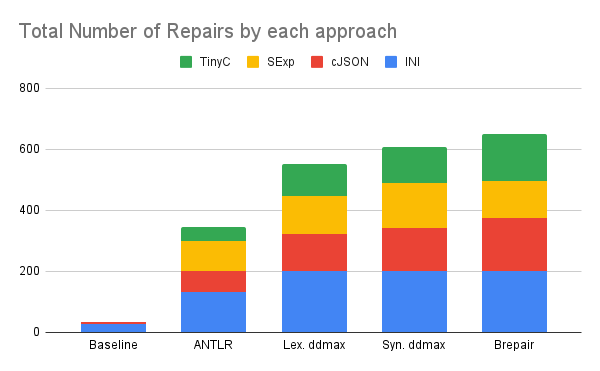
\includegraphics[width=0.45\textwidth]{figures/effectiveness.png}
\pgfplotstableread{
Label      INI    cJSON    SExpParser   TinyC
Baseline   27     6        0            0
ANTLR      133    69       96           46
Lex.ddmax  201    132      131          114
Syn.ddmax  201    144      149          120
FSynth     191    158      121          154
    }\effectivenessdata
\begin{minipage}{.45\textwidth}
\begin{tikzpicture}
\begin{axis}[
    ybar stacked,
    ymin=0,
    ymax=750,
    xtick=data,
    bar width=25,
    legend style={cells={anchor=west}, legend pos=north west},
    reverse legend=true,
    xticklabels from table={\effectivenessdata}{Label},
    xticklabel style={text width=2cm,align=center,font=\footnotesize},
    xtick style={draw=none},
]
    \addplot [fill=darkgray] table [y=INI, meta=Label, x expr=\coordindex] {\effectivenessdata};
    \addlegendentry{INI}
    \addplot [fill=gray] table [y=cJSON, meta=Label, x expr=\coordindex] {\effectivenessdata};
    \addlegendentry{cJSON}
    \addplot [fill=lightgray] table [y=SExpParser, meta=Label, x expr=\coordindex] {\effectivenessdata};
    \addlegendentry{SExpParser}
    \addplot [fill=white,nodes near coords,point meta=y] table [y=TinyC, meta=Label, x expr=\coordindex] {\effectivenessdata};
    \addlegendentry{TinyC}
\end{axis}
\end{tikzpicture}
\end{minipage}
\caption{Number of files repaired by each approach}
\label{fig:effectiveness}
%\vspace{-0.6cm}
\end{figure}

\end{document}
